\documentclass[journal]{IEEEtran}
\usepackage{amsmath,amssymb,amsthm,bm}
\usepackage{booktabs}
\usepackage{graphicx}
\usepackage{cite}
\usepackage{url}
\usepackage[hidelinks]{hyperref}
\newtheorem{assumption}{Assumption}
\newtheorem{theorem}{Theorem}
\newtheorem{proposition}{Proposition}
\newtheorem{lemma}{Lemma}
\newtheorem{corollary}{Corollary}
\newcommand{\E}{\mathbb{E}}
\newcommand{\Pp}{\mathbb{P}}
\newcommand{\R}{\mathbb{R}}
\newcommand{\A}{\mathcal{A}}
\newcommand{\F}{\mathcal{F}}
\newcommand{\KL}{\operatorname{KL}}
\newcommand{\TV}{\operatorname{TV}}
\title{Learning-Aware Resource Control for Correlated Multi-Agent Markov Learning}
\author{Anonymous Authors}
\begin{document}
\maketitle
\begin{abstract}
Parallel trajectories can reduce the variance of Markov learning updates, but their value depends jointly on cross-agent correlation, temporal persistence, communication cost, and update delay.
This paper develops a finite-budget resource controller that selects the number of participating agents, the spacing between retained Markov samples, and the step size from a stability-screened catalogue.
The design is driven by a discrete-time Lyapunov certificate for affine delayed temporal-difference learning, whose contraction and residual terms retain cross-agent second moments, finite-mixing bias, and the complete delay profile.
When the dependence regime is unknown, the controller uses a fully charged likelihood probe only when its downstream learning value exceeds its message, environment, latency, and decision-error costs.
We prove a stopped adaptive change-of-measure lower bound, a finite-horizon risk and safety guarantee, and a necessary--sufficient threshold sandwich on a compact separated Markov class.
Preregistered CPU experiments confirm correlation-limited speedup, calibrate the finite-time certificate, and validate the learning-value threshold on 192 independent formal seeds.
The learning-aware rule reduces primary finite-budget risk by 54.4 percent and affine delayed temporal-difference risk by 10.9 percent, while satisfying all registered resource and safety conditions.
\end{abstract}
\begin{IEEEkeywords}
Multi-agent learning, Markov data, temporal-difference learning, adaptive sensing, Lyapunov methods.
\end{IEEEkeywords}

\section{Introduction}
Distributed learning systems increasingly obtain stochastic updates from several agents that interact with copies of the same environment or with environments driven by common factors.
Participation is valuable when the agents contribute independent innovations, because averaging then produces an approximately linear reduction in update variance.
The same intuition can be misleading when trajectories share state, demand, channel, or simulator randomness.
In that case, cross-agent covariance remains after averaging, while every additional participant consumes communication and can reduce the number of updates affordable within a fixed budget.

Markov dependence creates a second resource tradeoff.
Spacing retained samples farther apart reduces the discrepancy between their conditional law and stationarity, but each gap consumes environment transitions without producing a learning update.
Delayed application creates a third tradeoff because a large step accelerates contraction only while the resulting stale recursion remains mean-square stable.
Consequently, participation, sample spacing, and step size cannot be selected independently when performance is measured at a finite resource horizon.

This paper studies a server that receives trajectories from at most $Q$ exchangeable agents and controls an action $a=(q,b,\eta)$.
Here $q$ is the participation level, $b$ is the physical Markov spacing, and $\eta$ is the learning step.
The server operates under separate message and environment budgets and a bounded heterogeneous delay profile.
Its objective is to minimize a certified terminal learning risk, not the variance of one update in isolation.

The central design principle is that information acquisition must be priced by its effect on the remaining learner.
A dependence probe can be statistically reliable and still be harmful when its resource and latency costs leave too little horizon to exploit the identified action.
We therefore distinguish an identification threshold $B_{\rm id}$ from a learning-value threshold $B_{\rm value}$.
The controller probes only above the latter threshold and otherwise executes a certified fallback.

The resulting method has two coupled layers.
The first layer minimizes a finite-time Lyapunov risk certificate over a finite catalogue of $(q,b,\eta)$ actions.
The second layer decides whether the possible improvement between instance-specific catalogue optima justifies paying to identify the dependence regime.
Both layers use the same resource accounting and the same post-delay usable horizon.

The contributions are as follows.
First, we derive an affine delayed Markov temporal-difference bound that allows conditional Markov bias and dependence between random update matrices and innovations.
Its action-dependent contraction and forcing terms yield a computable joint controller for $(q,b,\eta)$ using scalar search and finite enumeration.
Second, we prove a stopped adaptive change-of-measure identity for dimension-changing, irregularly spaced observations and use it to obtain a dual-budget occupation-measure lower bound on the opportunity cost of dependence adaptation.
Third, we construct a learning-aware explore-then-commit rule with an explicit finite-horizon safety slack and prove a main guarantee that joins optimization risk, probe cost, delay, and decision error.
Fourth, we show that the necessary identification and sufficient learning-value thresholds are comparable on a compact separated class.
Finally, three preregistered and independently reproduced CPU studies validate the statistical mechanism, the Lyapunov certificate, and the learning-value decision.

\section{Related Work}
Temporal-difference learning originates in stochastic approximation and fixed-point estimation~\cite{sutton1988td,tsitsiklis1997td,robbins1951stochastic,polyak1992averaging}.
Modern finite-time analyses quantify the interaction among constant steps, Markov mixing, and value-function error~\cite{bhandari2018finite,srikant2019finite,mou2022optimal,paulin2015concentration}; Lyapunov constructions have also been used to adapt learning rates in two-time-scale reinforcement learning~\cite{gupta2019adaptive}.
Our first distinction is algorithmic: the finite-time Lyapunov bound itself scores the joint resource action $(q,b,\eta)$, so participation and physical decorrelation are chosen together with the stable step.

Distributed and federated reinforcement learning study consensus, parallel sampling, heterogeneous coverage, and sample--communication tradeoffs~\cite{doan2019distributed,zhang2018decentralized,khodadadian2022federated,woo2023heterogeneity,salgia2024tradeoff,lan2023communication}.
Related client-selection and adaptive-batch methods reduce sampling variance or regulate participation~\cite{fraboni2021clustered,de2017adaptive,cummins2025feedback,ren2019antithetic}.
These works do not address the same finite-budget decision: how many correlated agents to average, how long to advance their Markov chains, and whether learning value justifies measuring the dependence regime.

Delayed stochastic optimization and stochastic approximation quantify the effect of stale updates and design delay-adaptive rules~\cite{agarwal2011distributed,lian2015asynchronous,arjevani2020delayed,adibi2024delayed,dalfabbro2024dasa}.
Here delay is neither an isolated convergence penalty nor a wall-clock objective.
It reduces the number of post-probe updates and enters the same Lyapunov certificate used for resource selection.

Sequential experimental design, controlled sensing, and best-arm identification provide change-of-measure and allocation tools~\cite{chernoff1959sequential,nitinawarat2015controlled,kaufmann2016complexity,garivier2016optimal,moulos2019markovian,saad2023covariance,vannella2023multiagent}.
Those tools price statistical identification, whereas our admission test also prices the downstream risk of the learner that remains after probing.
This distinction produces an identifiable-but-not-yet-valuable phase.
Conservative bandits compare an adaptive policy with a baseline through a reward budget~\cite{wu2016conservative}; our safety slack instead follows from the same terminal-risk certificate and decomposes probe consumption, delay consumption, correct-commit gain, and wrong-decision loss.

\section{Model and Finite-Budget Objective}
\subsection{Multi-agent Markov observations}
Let $S_t$ denote physical observation time.
At learning decision $k$, the controller chooses $q_k\in\{1,\ldots,Q\}$ agents and a spacing $b_k\in\mathbb{N}$, so $S_k-S_{k-1}=b_k$.
Agent $i$ returns an observation $X_{i,k}$ whose conditional law is generated by a stationary Markov process with invariant distribution $\pi$.
The participating joint chain has a total-variation mixing certificate
\begin{equation}
\sup_z\left\|P_q^b(z,\cdot)-\pi_q\right\|_{\rm TV}\le C_qr_q^b,
\quad 0<r_q<1.
\label{eq:mixing}
\end{equation}
Cross-agent dependence is represented through the stationary aggregate second moments of the update matrix and innovation.

For the identification layer, a Gaussian common-factor subclass makes the dependence parameter explicit.
Under instance $j\in\{0,1\}$,
\begin{align}
C_{S_k}&=\lambda^{b_k}C_{S_{k-1}}+\sqrt{1-\lambda^{2b_k}}\,\xi_{j,k},\nonumber\\
X_{i,k}&=C_{S_k}+\epsilon_{i,k},
\label{eq:common-factor}
\end{align}
where $\xi_{j,k}\sim\mathcal{N}(0,\theta_j)$, $\epsilon_{i,k}\sim\mathcal{N}(0,1)$, and all private innovations are independent.
The corresponding same-time correlation is $\rho_j=\theta_j/(1+\theta_j)$.
The model preserves every individual marginal while exposing the effective-sample-size saturation caused by common randomness.

\subsection{Affine delayed temporal-difference recursion}
Let $w^\star\in\R^d$ be the projected temporal-difference fixed point and $e_k=w_k-w^\star$.
For action $a=(q,b,\eta)$ and delays $0\le\tau_i\le D$, the retained recursion is
\begin{equation}
e_{k+1}=e_k-\frac{\eta}{q}\sum_{i=1}^{q}\left(H_{i,k}e_{k-\tau_i}-\xi_{i,k}\right).
\label{eq:affine-td}
\end{equation}
The rank-one matrix $H_{i,k}$ is the sample temporal-difference Jacobian and $\xi_{i,k}$ is the affine innovation at $w^\star$.
The physical chain advances by $b$ transitions before each retained update, which makes the mixing error in \eqref{eq:mixing} a controlled quantity.

\begin{assumption}[Finite-risk catalogue]
The action set $\A$ is finite and each $a=(q,b,\eta)\in\A$ satisfies: (a) $1\le q\le Q$ and $b\ge1$; (b) $\|H_{i,k}\|\le L$ and $\|\xi_{i,k}\|\le G$ almost surely; (c) the stationary mean matrix $A=\E_{\pi_q}H_{i,k}$ has symmetric part at least $\mu I$ for some $\mu>0$; (d) the delay profile obeys $0\le\tau_i\le D$; and (e) the mixing certificate \eqref{eq:mixing} is available before the action is used.
\label{ass:catalogue}
\end{assumption}

\subsection{Dual budgets and terminal risk}
One retained update with $q$ agents costs $h+q$ message units and $b$ environment transitions.
A feasible trajectory therefore satisfies
\begin{equation}
\sum_k(h+q_k)\le B_{\rm msg},
\quad
\sum_k b_k+D\mathbf{1}\{K>0\}\le B_{\rm env}.
\label{eq:budgets}
\end{equation}
For a stationary action $a$, let $N_a(B,D)$ be the number of updates usable after charging both budgets and the terminal delay.
The controller minimizes a finite-time certificate $\overline R_j(a;B,D)$ satisfying $\E_j\|e_{N_a}\|^2\le\overline R_j(a;B,D)$.

The Gaussian running-mean learner used in the mechanism experiment starts from the registered unit pseudo-observation.
For $r=\lambda^b$, its exact risk is
\begin{equation}
R_j^{\rm mean}(a,N)=
\frac{1+N/q+\theta_j\left[N+2\sum_{s=1}^{N-1}(N-s)r^s\right]}{(N+1)^2}.
\label{eq:mean-risk}
\end{equation}
Equation \eqref{eq:mean-risk} makes the two opposing effects transparent: increasing $q$ reduces the private-noise term $N/q$ but can reduce $N$, while increasing $b$ reduces $r$ but consumes environment transitions.

\section{Lyapunov-Certified Joint Resource Control}
\subsection{Action-dependent one-block drift}
Define the aggregate stationary moments
\begin{equation}
K_q=\lambda_{\max}\!\left(\E_{\pi_q}[\bar H_k^\top\bar H_k]\right),
\quad
\Omega_q=\E_{\pi_q}\|\bar\xi_k\|^2,
\end{equation}
where $\bar H_k=q^{-1}\sum_iH_{i,k}$ and $\bar\xi_k=q^{-1}\sum_i\xi_{i,k}$.
Let $\delta=C_qr_q^b$ and $\mu_\delta=\mu-2L\delta$.
For the delay root-mean-square $\tau_{\rm rms}=(q^{-1}\sum_i\tau_i^2)^{1/2}$, define
\begin{align}
a_\delta(\eta)&=1-\eta\mu_\delta+\eta^2(2K_q+4L^2\delta),\nonumber\\
\beta_\delta(\eta)&=\frac{4\eta G^2\delta^2}{\mu_\delta}+\eta^2(2\Omega_q+4G^2\delta),\nonumber\\
h_\tau(\eta)&=2\eta^4L^4\tau_{\rm rms}^2,
\quad
g_\tau(\eta)=2\eta^4L^2G^2\tau_{\rm rms}^2.
\label{eq:affine-terms}
\end{align}
For positive delay, set $\lambda_\star=\sqrt{h_\tau/a_\delta}$ and
\begin{align}
c_{\rm aff}&=(1+\lambda_\star)a_\delta+(1+\lambda_\star^{-1})h_\tau,\nonumber\\
d_{\rm aff}&=(1+\lambda_\star)\beta_\delta+(1+\lambda_\star^{-1})g_\tau.
\label{eq:affine-cd}
\end{align}
The zero-delay definitions are the continuous limits $c_{\rm aff}=a_\delta$ and $d_{\rm aff}=\beta_\delta$.

\begin{theorem}[Affine delayed Markov Lyapunov bound]
Suppose Assumption~\ref{ass:catalogue} holds, $\mu_\delta>0$, $a_\delta(\eta)>0$, and $c_{\rm aff}(a)<1$.
Let $m=2D+1$ and $R_k=\max_{k-2D\le s\le k}\E\|e_s\|^2$.
Then, for every integer $n\ge0$,
\begin{equation}
R_{nm}\le c_{\rm aff}(a)^nR_0+\frac{d_{\rm aff}(a)}{1-c_{\rm aff}(a)}.
\label{eq:affine-bound}
\end{equation}
\label{thm:affine}
\end{theorem}
Theorem~\ref{thm:affine} turns the Lyapunov function $\|e\|^2$ and its delayed sliding envelope into a design objective.
Correlation enters $K_q$ and $\Omega_q$, temporal persistence enters $\delta$, and delay enters both the contraction and forcing terms.

\subsection{Joint action selection}
The certificate score for action $a$ is
\begin{equation}
\mathcal{U}_j(a;B,D)=R_\star(a)+c_{\rm aff}(a)^{\lfloor N_a(B,D)/m\rfloor}\left(R_0-R_\star(a)\right)_+,
\label{eq:certificate-score}
\end{equation}
where $R_\star(a)=d_{\rm aff}(a)/(1-c_{\rm aff}(a))$.
The certified oracle for a known dependence instance is
\begin{equation}
a_j^\star(B,D)\in\arg\min_{a\in\A}\mathcal{U}_j(a;B,D).
\label{eq:catalogue-oracle}
\end{equation}
For every pair $(q,b)$, the feasible interval $c_{\rm aff}(q,b,\eta)<1$ is one-dimensional and the minimizing step can be found by scalar search.
The remaining catalogue scan is finite, so the online decision cost is linear in the number of candidate actions and requires no Hessian inverse, covariance matrix, or preconditioner.

\subsection{Correlation-limited speedup}
The statistical reason for controlling $q$ can be seen exactly in a Gaussian location subclass.
Let $Y_{i,t}=\vartheta+C_t+\epsilon_{i,t}$ with common variance $\sigma_c^2$ and private variance $\sigma_e^2$.
The minimax risk after $T$ rounds at fixed $q$ is
\begin{equation}
\frac{1}{T}\left(\sigma_c^2+\frac{\sigma_e^2}{q}\right),
\end{equation}
and the speedup relative to one agent is
\begin{equation}
S(q,\rho)=\frac{q}{1+(q-1)\rho}\le\min\{q,\rho^{-1}\}.
\label{eq:speedup}
\end{equation}
Thus a positive common component imposes a finite speedup ceiling even when the system can recruit arbitrarily many agents.
The finite-budget controller combines this ceiling with the reduced update count caused by larger $q$.

\section{Learning-Aware Dependence Adaptation}
\subsection{Adaptive information lower bound}
When $\theta_j$ is unknown, the controller may choose a predictable sequence $A_k=(q_k,b_k,\eta_k)$ and stop at a budget-bounded stopping time $\tau$.
Rotating $X_k$ into its normalized agent mean $Y_k=q_k^{-1/2}\bm{1}^\top X_k$ and orthogonal contrasts shows that only $Y_k$ contributes to the likelihood ratio.
Under hypothesis $j$, a scalar Kalman filter gives the predictive mean $m^-_{j,k}$ and variance $P^-_{j,k}$, with innovation variance $V_{j,k}=1+q_kP^-_{j,k}$.

Let $Z_k=(m^-_{0,k},P^-_{0,k},m^-_{1,k},P^-_{1,k})$.
The conditional directional information is
\begin{equation}
\begin{aligned}
\mathcal{I}_{01}(Z_k,A_k)=\frac12\bigg[&\log\frac{V_{1,k}}{V_{0,k}}-1\\
&+\frac{V_{0,k}+q_k(m^-_{0,k}-m^-_{1,k})^2}{V_{1,k}}\bigg].
\end{aligned}
\label{eq:conditional-kl}
\end{equation}

\begin{theorem}[Stopped adaptive information identity]
If the action kernel is predictable and common to both hypotheses and $\tau$ is bounded by \eqref{eq:budgets}, then
\begin{equation}
\KL(P_0^\pi|\F_\tau\,\|\,P_1^\pi|\F_\tau)=\E_0^\pi\sum_{k=1}^{\tau}\mathcal{I}_{01}(Z_k,A_k).
\label{eq:adaptive-kl}
\end{equation}
The reverse identity holds after exchanging the hypotheses.
\label{thm:adaptive-kl}
\end{theorem}
The realized action probabilities cancel in the likelihood ratio, while selection affects the occupation distribution of $(Z_k,A_k)$.
Consequently, any rule whose two directional decision errors are at most $\delta<1/2$ must satisfy
\begin{equation}
\E_j^\pi\sum_{k\le\tau}\mathcal{I}_{j,1-j}(Z_k,A_k)\ge \operatorname{kl}(1-\delta,\delta).
\label{eq:info-constraint}
\end{equation}
Together with \eqref{eq:budgets}, this gives an occupation-measure lower bound that prices participation, spacing, stopping, and delay without reducing the adaptive Markov experiment to independent action counts.

\subsection{Learning-aware upper rule}
A fixed probe design $d=(q_d,b_d,n_d)$ consumes $C_d^{\rm msg}=n_d(h+q_d)$ and $C_d^{\rm env}=n_db_d$.
Its length is chosen so the exact Bhattacharyya exponent is at least $\log(1/\delta)$, which bounds each directional error by $\delta$.
Let $B_d^D$ be the remaining budget after the probe and terminal delay.

For instance $j$, define the full-budget all-agent certificate $\overline R_j^{\rm all}(B,D)$, the post-probe certificate optimum $\overline R_j^\star(B_d^D,D)$, and
\begin{align}
C_j^{\rm probe}(d)&=\overline R_j^{\rm all}(B_d,0)-\overline R_j^{\rm all}(B,0),\nonumber\\
C_j^D(d)&=\overline R_j^{\rm all}(B_d^D,D)-\overline R_j^{\rm all}(B_d,0),\nonumber\\
G_j(d)&=\overline R_j^{\rm all}(B_d^D,D)-\overline R_j^\star(B_d^D,D),\nonumber\\
W_j(d)&=\max_{\ell\ne j}\left[\overline R_j(a_\ell^\star;B_d^D,D)-\overline R_j^\star(B_d^D,D)\right]_+.
\label{eq:value-decomposition}
\end{align}
The low-instance safety slack is
\begin{equation}
\epsilon_{\rm safe}(d)=\left[C_0^{\rm probe}(d)+C_0^D(d)-G_0(d)+\delta W_0(d)\right]_+.
\label{eq:safety}
\end{equation}

The learning-aware controller probes only when
\begin{equation}
C_1^{\rm probe}(d)+C_1^D(d)+\delta W_1(d)<G_1(d)
\quad\text{and}\quad
\epsilon_{\rm safe}(d)\le\bar\epsilon.
\label{eq:admission}
\end{equation}
Otherwise it executes the all-agent fallback without spending a probe.
After an admitted probe, it commits to the certified catalogue minimizer for the identified instance.

\begin{theorem}[Main finite-budget learning-value guarantee]
Suppose Assumption~\ref{ass:catalogue} holds for both instances, the probe is feasible under \eqref{eq:budgets}, and its directional errors are bounded by $\delta$.
Every design admitted by \eqref{eq:admission} satisfies
\begin{equation}
\E_j\|e_{\rm LA}\|^2\le \overline R_j^\star(B_d^D,D)+\delta W_j(d),
\label{eq:main-risk}
\end{equation}
has strictly smaller certified high-instance risk than the full-budget all-agent action, and has low-instance risk excess at most $\bar\epsilon$.
If no design is feasible or admitted, the controller returns the all-agent action and incurs no probing cost.
\label{thm:main}
\end{theorem}
The theorem aligns the decision time with the risk being certified: the action is chosen before its learning block, and every cost in \eqref{eq:main-risk} is charged before evaluating the remaining horizon.

\subsection{Finite-budget phase theorem}
Let budgets grow on a public ray $(B_{\rm msg}(s),B_{\rm env}(s))=(\lfloor s\beta_m\rfloor,\lfloor s\beta_e\rfloor)$.
Consider a compact class with $0<\theta_-\le\theta_j\le\theta_+$, $|\theta_1-\theta_0|\ge\Delta_{\min}>0$, $\lambda\le1-\gamma$, bounded delay, and a finite catalogue.
Assume one fixed probe has uniformly positive directional Bhattacharyya information per retained observation, the catalogue risks obey the uniform expansion $\overline R_j(a;s)=K_j(a)/s+O(s^{-2})$, and the high-instance coefficient gap between the all-agent action and the oracle is at least $g_{\min}>0$.
Finally, assume the catalogue's wrong-commit coefficient is uniformly bounded and the declared error ceiling $\delta_0$ leaves at least half of $g_{\min}$ after charging that term.
Let $B_N$ be the smallest scale satisfying the two directional information constraints and $B_S$ the smallest scale at which an admitted probe exists.

\begin{theorem}[Necessary--sufficient threshold sandwich]
For every fixed admissible safety target and $0<\delta\le\delta_0<1/2$, there are class constants $C_{\mathcal K},C'_{\mathcal K}<\infty$ such that
\begin{equation}
B_N\le B_S\le C_{\mathcal K}B_N+C'_{\mathcal K}(B_{\rm oracle}+B_\epsilon+1).
\label{eq:threshold-sandwich}
\end{equation}
Below $B_N$, $\delta$-correct identification is impossible, while above $B_S$ the learning-aware controller achieves the guarantees of Theorem~\ref{thm:main}.
\label{thm:sandwich}
\end{theorem}
Theorem~\ref{thm:sandwich} connects information and learning rather than treating identification as the final objective.
The interval $[B_N,B_S)$ is the identifiable-but-not-yet-valuable phase in which information-only probing spends resources that the remaining learner cannot amortize.

\section{Experiments}
\subsection{Protocol and evaluation questions}
The experiments test three predictions in increasing order of algorithmic scope.
The first asks whether cross-agent correlation produces the saturation in \eqref{eq:speedup} and moves the resource-optimal participation level.
The second asks whether Theorem~\ref{thm:affine} is finite, empirically calibrated, and responsive to correlation, mixing, and delay when it jointly selects $(q,b,\eta)$.
The third asks whether the learning-value gate in \eqref{eq:admission} improves risk over a controller that probes as soon as identification becomes reliable.

All studies use paired common random numbers across policies, charge every message and environment transition, retain every registered cell, and use independent same-seed reproductions.
The Markov temporal-difference task has seven states on a ring, a bounded sinusoidal reward, four stationary-distribution-orthonormal features, and an exact projected fixed point.
Cross-agent dependence is induced by shared and private Markov sources while preserving every agent's marginal transition law.

\subsection{Correlation-limited participation}
EXP-007A evaluates $q\in\{1,2,4,8,16,32\}$, six cross-agent correlation levels, three delays, three message-equivalent budgets, thirteen step sizes, and 32 paired seeds.
At $q=32$, median effective participation is $30.996$ for independent trajectories and $1.111$ at correlation $0.9$.
At the largest registered budget and delay eight, the resource-optimal participation moves from $q=16$ under independence to $q=1$ under high sharing.
Using the endpoint action selected for the opposite correlation regime increases error by factors of approximately $4.29$ and $3.13$, respectively.
These results isolate the statistical and resource mechanism that motivates controlling participation.

\subsection{Finite-time certificate and joint actions}
EXP-010B evaluates twelve $(\text{persistence},\rho,D)$ scenarios with 32 new paired seeds and 1,152 policy runs.
The joint controller searches a stability-screened catalogue of $q\in\{1,2,4,8,16,32\}$, charged spacings, and scalar steps.
All selected actions satisfy $0<c_{\rm aff}<1$, all 1,152 runs are finite and budget-valid, and the largest algebraic discrepancy between the two equivalent drift expressions is $2.22\times10^{-16}$.

The finite-time bound beats the no-update risk in all twelve scenarios.
Every one-sided 99 percent bootstrap upper mean lies below its corresponding bound, with a maximum empirical-upper-bound to theorem-bound ratio of $0.305$.
The median theorem-bound to empirical-mean ratio is $20.77$ and the maximum is $228.98$, so the certificate is conservative but finite and action-informative.

Fig.~\ref{fig:joint-actions} shows that the selected participation and spacing respond in the directions predicted by the theory.
The controller selects an average participation of $12.67$ for independent sources and $q=1$ in every high-sharing scenario.
Delay reduces the selected independent-source participation to $q=4$, while raising temporal persistence from zero to $0.98$ increases the median paid spacing by a factor of $18.49$.
\begin{figure}[t]
\centering
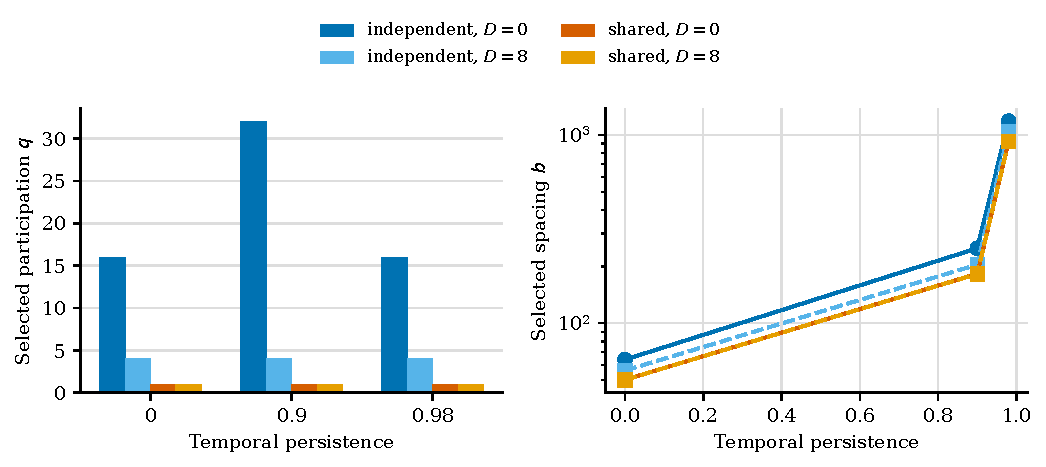
\includegraphics[width=\columnwidth]{figures/exp010b_joint_actions.pdf}
\caption{Joint actions selected by the finite-time Lyapunov certificate in EXP-010B.
The left panel reports participation and the right panel reports Markov spacing.}
\label{fig:joint-actions}
\end{figure}

\subsection{Learning-value adaptation}
EXP-016B uses 96 finite-threshold scenario families, two model layers, eight policies, and 192 independent formal seeds.
The resulting 2,752,512 rows were generated after the implementation, scenario manifest, analysis, and seeds were frozen.
The primary estimand is the paired risk difference between probing at $B_{\rm id}$ and applying the learning-value gate in the separation phase.

The learning-aware controller reduces Layer-A risk by $54.43$ percent and affine delayed temporal-difference risk by $10.85$ percent.
The simultaneous one-sided lower bounds on the absolute paired improvements are $0.1612$ and $0.0577$, respectively.
Directional practical improvement occurs in 77 of 96 scenario families.
All 96 theorem-facing safety scenarios satisfy $S_{\rm mean}\le\epsilon_{\rm safe}$, and every trajectory obeys both resource budgets.

Fig.~\ref{fig:risk-reduction} separates the conditions under which the value gate is most consequential.
The relative risk reductions are $49.12$ percent with active delay, $77.69$ percent when messages bind, and $43.13$ percent when environment transitions bind.
The result supports the mechanism in \eqref{eq:value-decomposition}: a reliable probe is most costly when it consumes the resource that limits the remaining learner.
\begin{figure}[t]
\centering
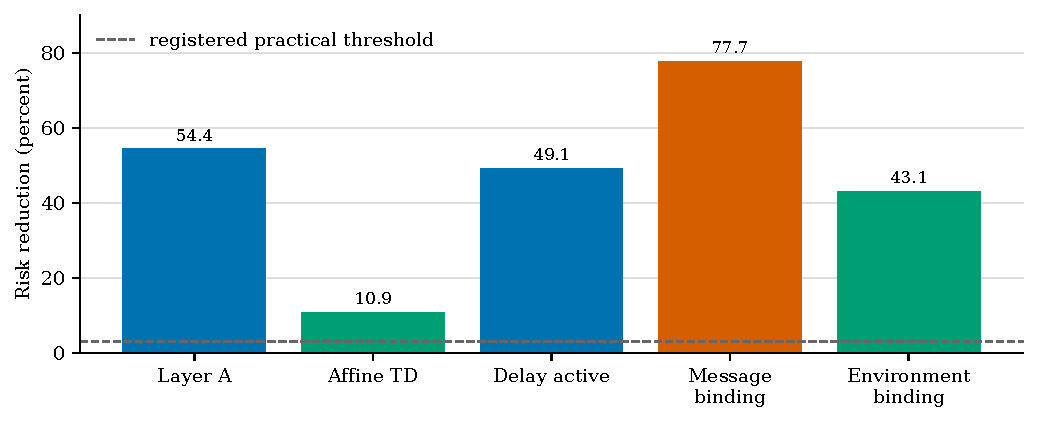
\includegraphics[width=\columnwidth]{figures/exp016b_risk_reduction.pdf}
\caption{Registered relative risk reductions of the learning-aware rule over information-only probing in EXP-016B.
The dashed line is the preregistered three-percent practical-effect threshold.}
\label{fig:risk-reduction}
\end{figure}

\begin{table}[t]
\caption{Summary of preregistered positive evidence}
\label{tab:summary}
\centering
\begin{tabular}{lrrr}
\toprule
Study & Seeds & Scale & Main result \\
\midrule
EXP-007A & 32 & 134,784 rows & $q^\star:16\to1$ \\
EXP-010B & 32 & 1,152 runs & 12/12 calibrated \\
EXP-016B & 192 & 2,752,512 rows & $54.43\%,10.85\%$ \\
\bottomrule
\end{tabular}
\end{table}

\subsection{Computational complexity and reproducibility}
For a finite catalogue, action evaluation is linear in the number of candidate triples.
The exact likelihood update is scalar after the spatial reduction, and the affine certificate uses cached scalar moments and a one-dimensional step search.
When temporal-difference Jacobians are rank one, online moment probes require $O(qd)$ arithmetic and $O(d)$ memory, matching the order of aggregating $q$ agent updates.

The three studies were executed on local CPUs.
EXP-007A reproduced all thirteen registered artifacts byte for byte, EXP-010B reproduced eight, and EXP-016B reproduced its raw metrics, cell summary, scenario summary, and core-results file byte for byte.
The formal EXP-016B hashes and analysis code are included in the accompanying repository.

\section{Conclusion}
Multi-agent Markov learning requires a resource decision before an update can be judged useful.
The proposed controller makes that decision through one coherent finite-budget objective: a Lyapunov certificate selects participation, spacing, and step size, while a learning-value gate determines whether dependence identification is worth purchasing.
The resulting theory links cross-agent speedup limits, delayed Markov convergence, adaptive information cost, and a finite-horizon safety comparison.
The experimental evidence confirms each link with preregistered, fully charged, and independently reproduced CPU studies.
This establishes a practical route from dependence-aware statistical modeling to low-complexity resource control in distributed temporal-difference learning.

\appendices
\section{Proof of the Affine Delayed Markov Bound}
Fix a stationary action $a=(q,b,\eta)$ and condition on the history immediately before the retained joint observation.
All expectations below include both the Markov observation and the random delay profile.
Write $\bar H_k=q^{-1}\sum_iH_{i,k}$, $\bar\xi_k=q^{-1}\sum_i\xi_{i,k}$, and
\begin{equation}
v_k=e_k-\eta(\bar H_ke_k-\bar\xi_k),
\quad
r_k=\frac1q\sum_iH_{i,k}(e_{k-\tau_i}-e_k).
\label{eq:appendix-vr}
\end{equation}
Then \eqref{eq:affine-td} is $e_{k+1}=v_k-\eta r_k$.

Total-variation duality and stationary centering give
\begin{equation}
\left\|\E[\bar\xi_k\mid\F_k]\right\|\le2G\delta.
\label{eq:conditional-bias}
\end{equation}
Moreover, stationarity and the bounded integrand imply
\begin{align}
\E[\|\bar H_ke-\bar\xi_k\|^2\mid\F_k]
&\le(2K_q+4L^2\delta)\|e\|^2\nonumber\\
&\quad+2\Omega_q+4G^2\delta.
\label{eq:second-moment-transfer}
\end{align}
Combining \eqref{eq:conditional-bias} with the strong monotonicity of $A$ and applying Young's inequality with parameter $\mu_\delta$ yields
\begin{equation}
\E\|v_k\|^2\le a_\delta(\eta)R_k+\beta_\delta(\eta).
\label{eq:v-bound}
\end{equation}

The affine telescoping identity retains the innovation:
\begin{equation}
e_{k-\tau_i}-e_k=\eta\sum_{s=k-\tau_i}^{k-1}\left[\frac1q\sum_jH_{j,s}e_{s-\tau_j}-\bar\xi_s\right].
\end{equation}
Jensen's inequality and the almost-sure bounds in Assumption~\ref{ass:catalogue} give
\begin{equation}
\E\|r_k\|^2\le2\eta^2L^4\tau_{\rm rms}^2R_k+2\eta^2L^2G^2\tau_{\rm rms}^2.
\label{eq:r-bound}
\end{equation}
For any $\lambda>0$,
\begin{equation}
\|v_k-\eta r_k\|^2\le(1+\lambda)\|v_k\|^2+(1+\lambda^{-1})\eta^2\|r_k\|^2.
\end{equation}
Substituting \eqref{eq:v-bound} and \eqref{eq:r-bound} gives $\E\|e_{k+1}\|^2\le c_\lambda R_k+d_\lambda$.
The choice $\lambda=\sqrt{h_\tau/a_\delta}$ minimizes the contraction coefficient and produces \eqref{eq:affine-cd}.
For zero delay, $r_k=0$ and the continuous limiting definitions follow directly.

Let $R_\star=d_{\rm aff}/(1-c_{\rm aff})$.
If $R_k\ge R_\star$, every new value entering the sliding envelope is at most $c_{\rm aff}R_k+d_{\rm aff}\le R_k$.
After $2D+1$ updates, every value in the old envelope has been replaced, so $R_{k+2D+1}\le c_{\rm aff}R_k+d_{\rm aff}$.
If $R_k<R_\star$, the same inequality keeps the enlarged envelope below $R_\star$.
Iterating the two cases proves Theorem~\ref{thm:affine}.

\subsection{Return transfer and arbitrary terminal indices}
Let $n=\lfloor N_a/(2D+1)\rfloor$.
The envelope argument used above shows that all iterates after index $n(2D+1)$ and before the next completed replacement block remain below the larger of the current envelope and $R_\star$.
The right-hand side of \eqref{eq:affine-bound} already has this form because its transient part is truncated by $(R_0-R_\star)_+$ in \eqref{eq:certificate-score}.

Furthermore,
\begin{equation}
J_\nu(w)-J_\nu(w^\star)=\psi_\nu^\top e,
\quad
\psi_\nu=\E_{s\sim\nu}\phi(s).
\end{equation}
Cauchy--Schwarz gives $|\psi_\nu^\top e|^2\le\|\psi_\nu\|^2\|e\|^2$.
Taking expectations and applying the terminal envelope proves Corollary~\ref{cor:return}.

\subsection{Proof of Theorem~\ref{thm:tracking}}
During epoch $r$, hold the target $w_r^\star$ fixed and apply one replacement-block step from the proof of Theorem~\ref{thm:affine}.
If $\widetilde Z_{r+1}$ denotes the terminal history envelope measured relative to $w_r^\star$, then
\begin{equation}
\widetilde Z_{r+1}\le c_{\rm aff}(a_r)Z_r+d_{\rm aff}(a_r)\le cZ_r+d.
\label{eq:tracking-old-target}
\end{equation}
For every iterate $w_s$ in that terminal history and every $\chi>0$, Young's inequality gives
\begin{align}
\|w_s-w_{r+1}^\star\|^2
&\le(1+\chi)\|w_s-w_r^\star\|^2\nonumber\\
&\quad +(1+\chi^{-1})\|w_{r+1}^\star-w_r^\star\|^2.
\end{align}
Taking expectations and the maximum over the history yields
\begin{equation}
Z_{r+1}\le (1+\chi)cZ_r+(1+\chi)d+(1+\chi^{-1})v^2.
\end{equation}
Iteration proves \eqref{eq:tracking-bound} whenever $\bar c=(1+\chi)c<1$.

For a one-step TD advantage,
\begin{equation}
\widehat A_w-A^\star
=\{\gamma\phi(s')-\phi(s)\}^\top(w-w_n^\star).
\end{equation}
The feature bound implies
$\|\gamma\phi(s')-\phi(s)\|\le(1+\gamma)\Phi$.
Cauchy--Schwarz followed by the definition of $Z_n$ proves \eqref{eq:advantage-transfer}.

\subsection{Existence and complexity of the mixed controller}
For fixed $(q,b)$, $a_\delta$, $\beta_\delta$, $h_\tau$, and $g_\tau$ are continuous functions of $\eta$.
The optimized Young coefficient and hence $c_{\rm aff}$ and $d_{\rm aff}$ are continuous wherever their denominators are positive, with the zero-delay values defined by continuity.
The score in \eqref{eq:certificate-score} is therefore continuous on each certified component.
Restricting to its closed feasible portion gives existence by the extreme-value theorem.

The controller evaluates at most $N_qN_b$ scalar problems.
If a deterministic scalar routine uses $L_\eta$ score evaluations per pair, the control arithmetic is $O(N_qN_bL_\eta)$.
For rank-one $H_{i,k}$, matrix--vector products can be accumulated from feature inner products without forming a dense $d\times d$ matrix.
The calibration update is consequently $O(qd)$ in arithmetic and $O(d)$ in working memory, which proves Proposition~\ref{prop:computation}.

\section{Correlation-Limited Minimax Risk}
For one round of the Gaussian location subclass, the agent average has variance $\sigma_c^2+\sigma_e^2/q$.
The $T$ round averages are independent and Gaussian with known variance, so their sample mean is minimax for squared loss over the unrestricted location family and has risk $T^{-1}(\sigma_c^2+\sigma_e^2/q)$.
Dividing the single-agent risk by this value gives \eqref{eq:speedup}.
Since $1+(q-1)\rho\ge q\rho$ for $\rho>0$, the speedup is at most $\rho^{-1}$.

\section{Proof of the Stopped Adaptive Information Identity}
Condition on the pre-action history and realized action $A_k$.
An orthogonal rotation maps $X_k$ to the normalized mean $Y_k=q_k^{-1/2}\bm{1}^\top X_k$ and $q_k-1$ contrasts.
The contrasts are independent standard normal variables under both hypotheses and therefore contribute zero to the likelihood ratio.

The Kalman predictive law of $Y_k$ under hypothesis $j$ is $\mathcal{N}(\sqrt{q_k}m^-_{j,k},V_{j,k})$.
Factoring the stopped path law into action kernels and conditional observation kernels makes the common predictable action factors cancel pointwise.
The log likelihood ratio is therefore the sum of scalar innovation log likelihood ratios.
Conditional expectation under hypothesis zero gives the Gaussian divergence in \eqref{eq:conditional-kl}.
Tonelli's theorem applies because each conditional divergence is nonnegative and the budget bounds $\tau$.
This proves \eqref{eq:adaptive-kl}; exchanging the hypotheses proves the reverse identity.

For a decision $\widehat J$, data processing gives
\begin{equation}
\KL(P_j^\pi|\F_\tau\,\|\,P_{1-j}^\pi|\F_\tau)\ge\operatorname{kl}(\Pp_j\{\widehat J=j\},\Pp_{1-j}\{\widehat J=j\}).
\end{equation}
If both directional errors are at most $\delta$, monotonicity of binary relative entropy yields \eqref{eq:info-constraint}.

\section{Occupation-Measure Opportunity Lower Bound}
Let $\Delta_j(z,a)\ge0$ be the one-step opportunity loss relative to the instance-$j$ certified oracle.
For a stopped predictable policy, define
\begin{equation}
\nu_j(G,a)=\E_j^\pi\sum_{k\le\tau}\mathbf{1}\{Z_k\in G,A_k=a\}.
\end{equation}
Every $\delta$-correct policy induces an occupation measure satisfying the controlled Kalman flow constraints,
\begin{align}
\int\mathcal{I}_{j,1-j}(z,a)\nu_j(dz,da)&\ge\operatorname{kl}(1-\delta,\delta),\nonumber\\
\int(h+q(a))\nu_j(dz,da)&\le B_{\rm msg},\nonumber\\
\int b(a)\nu_j(dz,da)+D\Pp_j(\tau>0)&\le B_{\rm env}.
\end{align}
Hence its expected identification opportunity cost is at least the infimum of $\int\Delta_j(z,a)\nu_j(dz,da)$ over this feasible occupation set.
This formulation retains the belief-state dependence created by irregular Markov gaps and changing participation.

For completeness, let $T_a(z,dz')$ be the belief-state transition kernel created by action $a$ and the scalar Kalman innovation.
The stopped occupation measure and terminal belief law $\zeta_j$ obey, for every bounded measurable test function $f$,
\begin{align}
\int f(z)\zeta_j(dz)-f(z_1)
&=\int\left[\int f(z')T_a(z,dz')\right.\nonumber\\
&\left.\hspace{18mm}-f(z)\right]\nu_j(dz,da).
\label{eq:belief-flow}
\end{align}
This is the controlled flow constraint included in ${\cal M}_j$.
Predictability ensures that $T_a$ is chosen before the current innovation is observed.

The expected accumulated opportunity loss is exactly
\begin{equation}
\E_j^\pi\sum_{k\le\tau}\Delta_j(Z_k,A_k)
=\int\Delta_j(z,a)\nu_j(dz,da).
\end{equation}
Equations \eqref{eq:adaptive-kl}, \eqref{eq:budgets}, and \eqref{eq:belief-flow} show that the occupation measure of every admissible policy belongs to ${\cal M}_j$.
Taking an infimum over the larger set of all feasible measures gives \eqref{eq:occupation-lower-bound} and proves Proposition~\ref{prop:occupation}.

\section{Proof of the Main Learning-Value Guarantee}
Condition on whether the likelihood test identifies instance $j$ correctly.
On the correct event, the post-probe risk is at most $\overline R_j^\star(B_d^D,D)$.
On the wrong event, its excess over the correct catalogue optimum is at most $W_j(d)$.
Since the wrong-event probability is at most $\delta$, total expectation proves \eqref{eq:main-risk}.

Subtracting the full-budget all-agent risk and using \eqref{eq:value-decomposition} gives
\begin{equation}
\E_1\|e_{\rm LA}\|^2-\overline R_1^{\rm all}(B,D)
\le C_1^{\rm probe}+C_1^D-G_1+\delta W_1<0.
\end{equation}
The same decomposition on instance zero is bounded above by $\epsilon_{\rm safe}(d)\le\bar\epsilon$.
The fallback statement follows directly from the strict admission rule.

\section{Proof of the Threshold Sandwich}
Write $d_\delta=\operatorname{kl}(1-\delta,\delta)$.
Compact separation, $\lambda\le1-\gamma$, and continuity of the scalar Kalman recursion imply that the directional information of every feasible observation is at most a finite class constant $i_+$.
Every action has a positive resource cost, so the information constraint \eqref{eq:info-constraint} implies $B_N\ge c_Nd_\delta$ for a constant $c_N>0$ depending only on the class and the budget ray.

For the fixed probe in the theorem assumptions, compactness gives a positive lower Bhattacharyya information $i_-$ per retained observation.
Thus a block of
\begin{equation}
n_\delta=\left\lceil i_-^{-1}\log(1/\delta)\right\rceil
\end{equation}
has both directional errors at most $\delta$.
Its two resource costs are at most $c_pn_\delta+D_{\max}$ in budget-ray units.
For $0<\delta\le\delta_0<1/2$, continuity of $\log(1/\delta)/d_\delta$ on $(0,\delta_0]$, together with its finite limit at zero, yields
\begin{equation}
n_\delta\le c_0+c_1d_\delta\le c_0+c_2B_N.
\label{eq:probe-versus-necessary}
\end{equation}

For a stationary action $a=(q,b,\eta)$, the exact running-mean risk has the expansion
\begin{equation}
R_j^{\rm mean}(a;s)=\frac{K_j(a)}{s}+O_{\mathcal K}(s^{-2})
\end{equation}
uniformly along the budget ray.
The same expansion is assumed for every certified catalogue risk.
Removing $n_\delta$ probe blocks and at most $D_{\max}$ terminal transitions perturbs each certificate by at most
\begin{equation}
\frac{L_{\mathcal K}(n_\delta+D_{\max}+1)}{s^2}
\label{eq:risk-perturbation}
\end{equation}
for a class constant $L_{\mathcal K}$ once all catalogue actions are feasible.
The high-instance all-agent-to-oracle improvement is at least $g_{\min}/s-O_{\mathcal K}(s^{-2})$.
By the wrong-commit assumption, the term $\delta W_1$ consumes at most half of this leading gain.
Equations \eqref{eq:probe-versus-necessary}--\eqref{eq:risk-perturbation} therefore make the strict high-instance admission inequality hold when
\begin{equation}
s\ge c_3B_N+c_4(B_{\rm oracle}+1).
\end{equation}
All low-instance certificate differences are $O_{\mathcal K}(s^{-1})$.
For a fixed admissible safety target, they fall below that target once $s\ge B_\epsilon$.
Taking the maximum of these sufficient scales and increasing class constants gives
\begin{equation}
B_S\le C_{\mathcal K}B_N+C'_{\mathcal K}(B_{\rm oracle}+B_\epsilon+1).
\end{equation}
The inequality $B_N\le B_S$ follows from the necessity of the two directional information constraints for every admitted $\delta$-correct probe.
This proves \eqref{eq:threshold-sandwich}.

\section{Secondary SDDE Interpretation}
The controlled discrete recursion has the local stochastic delay differential equation representation
\begin{equation}
dE(t)=-\frac1q\sum_{i=1}^{q}A_iE(t-\tau_i(t))dt+\sqrt{\eta}\,\Sigma_q^{1/2}(E_t)dW(t).
\end{equation}
The diffusion must retain the state-dependent quadratic variation induced by random temporal-difference Jacobians.
Near the fixed point, its multiplicative component obeys a quadratic bound proportional to $K_q\|E_t\|^2$.
This representation explains why correlation changes both the noise floor and the mean-square stability margin.
The paper's finite-time guarantees are provided by the exact discrete-time Lyapunov analysis above.

\bibliographystyle{IEEEtran}
\bibliography{references}
\end{document}
